%
% ####################################################################################################################################################################################
% ####################################################################################################################################################################################
% ####################################################################################################################################################################################
% ####################################################################################################################################################################################
%

\documentclass[]{myHOWTO-V001}

%
% ####################################################################################################################################################################################
% ####################################################################################################################################################################################
%

\usepackage{myTCB-V001}

%
% ####################################################################################################################################################################################
% ####################################################################################################################################################################################
%

\title{The \textbf{myTCB-V1} Package\\{\small Text and Listing Boxes}}
\version{1.00}
\author{Norbert EHART (norbert@ehart.net)}
\date{\today}

%
% ####################################################################################################################################################################################
% ####################################################################################################################################################################################
% ####################################################################################################################################################################################
% ####################################################################################################################################################################################
%

\begin{document}

%
% ####################################################################################################################################################################################
% ####################################################################################################################################################################################
%

\selectlanguage{english}

%
% ####################################################################################################################################################################################
% ####################################################################################################################################################################################
%

\maketitle

%
% ####################################################################################################################################################################################
% ####################################################################################################################################################################################
%

\tableofcontents

%
% ####################################################################################################################################################################################
% ####################################################################################################################################################################################
%

\section{Introduction}

Latex is heavily used in scientific fields, such as electrical engineering, mechanical engineering, and computer science. Especially in these areas, it is sometimes necessary that certain sections of the text are displayed inside a box. This box can, but does not have to, differ from the standard colors of the text.

\begin{myBOX}{title={This is an example box}}
\lipsum[4]
\end{myBOX}

In computer science, for example, it is very often necessary to display sections of configuration or program code.

\begin{myCODE}{listing options={language=python, style=number, firstnumber=1}, title={A simple Python Program}}
#
# Python Example
#

print("Hi, This is an example program")

i = 0

while i < 10:
	print(i)
	i=i+1
\end{myCODE}

For this purpose, it is necessary to tell Latex that certain sections should not be interpreted as normal text.

The \emph{myTCB-V1} package provides an environment for text and listing boxes. A text box is a paragraph-making environment that produces normal text (including pictures, etc...) with automatic
word splitting, line and page breaking to fit the texts within a specified area. A listing box is a paragraph-making environment that gets \LaTeX{} to print exactly what you type. It transforms \LaTeX{} into a typewriter, where carriage returns and whitespaces will have the same effect as with a typewriter. The output looks exactly as it looks in the input file.

\pagebreak

The \emph{myTCB-V1} package loads automatically the packages shown in \styref{loadingpackages}.

\begin{mySTYdoclst}{Packages}{label={sty:loadingpackages}}
\RequirePackage{lipsum}

\RequirePackage{graphicx}
\RequirePackage{wrapfig}

\RequirePackage{xcolor}

\RequirePackage{verbatim}
\RequirePackage{fancyvrb}
\RequirePackage{listings}

\RequirePackage{float}

\RequirePackage{refstyle}

\RequirePackage{tcolorbox}
	\tcbuselibrary{skins,breakable,listings,xparse}
\end{mySTYdoclst}

To load the package, write \Verb|\usepackage{myTCB-V1}| in the preamble of your document. To use this package, it is highly recommended to have the complete \LaTeX{} distribution installed. This will avoid problems with dependencies.

\begin{myTEXEXdoclst}{Loading myTCB-V1}{label={texex:loadingmyTCBv1}}
\usepackage{myTCB-V1}
\end{myTEXEXdoclst}

%
% ####################################################################################################################################################################################
% ####################################################################################################################################################################################
%

\section{The Text Environment without a List Index}

The \emph{myTCB-V1} package has a predefined environment, which is called \Verb|myBOX|. In this environment there is no list index available and only text boxes are created

\begin{myTEXEXdoclst}{myBOX without a List Entry}{label={texex:myboxwolistent}, listing and text}
\begin{myBOX}{}
	\lipsum[3]
\end{myBOX}
\end{myTEXEXdoclst}

A title can be submitted as an optional argument, which appears in the upper right corner of the box.

\begin{myTEXEXdoclst}{myBOX without a List Entry and with a Title}{label={texex:myboxwolistentwtitle}, listing and text}
\begin{myBOX}{title={This is myBOX}}
	\lipsum[4]
\end{myBOX}
\end{myTEXEXdoclst}

%
% ####################################################################################################################################################################################
% ####################################################################################################################################################################################
%

\section{The Text Environment with a List Index}

The \emph{myTCB-V1} package has a predefined environment, which is called \Verb|myBOXlst|. In this environment there is a list index available and only text boxes are created. A title (\verb|TITLE1|) must be passed as a mandatory argument. This title does not appear on the box, instead it is found in the list index. The box itself is titled with \emph{MyBOX} and a sequential number.

\begin{myTEXEXdoclst}{myBOX with a List Entry}{label={texex:myboxwithlistent}, listing and text}
\begin{myBOXlst}{TITLE1}{}
	\lipsum[4]
\end{myBOXlst}
\end{myTEXEXdoclst}

\begin{minipage}{0.46\linewidth}
\centering
\begin{myFIGlst}{myBOX LoF}{label={fig:myboxlofdef}}
	\includegraphics[page=1,scale=0.18]{examples/myBOXV000.pdf}
\end{myFIGlst}
\end{minipage}
\begin{minipage}{0.46\linewidth}
You can create the list index with the command \Verb|\listofmyBOX|.

\begin{myTEXEXdoclst}{List Entries of MySTY}{label={texex:mystylistentry}, listing only}
\listofmyBOX
\end{myTEXEXdoclst}

This will create a list index which looks like the picture in \figref{myboxlofdef}. 
\end{minipage}

If you want to change the horizontal spacing of the list entries, you can do this quite simple with the following code in the preamble, which is illustrated in \texexref{remleadnumbmybox}.

\begin{myTEXEXdoclst}{Altering the List Index Spacing of myBOXlst}{label={texex:remleadnumbmybox}, listing only}
\makeatletter
	\renewcommand{\l@myBOX}{\@dottedtocline{1}{0mm}{0mm}}
\makeatother
\end{myTEXEXdoclst}

If you want to change the vertical spacing of the list entries, you can do this quite simple with the following code in the preamble, which is illustrated in \texexref{remleadnumbmyboxhori}.

\begin{myTEXEXdoclst}{Altering the List Index Spacing of myBOXlst}{label={texex:remleadnumbmyboxhori}, listing only}
\makeatletter
	\addtocontents{myBOX}{\protect\vspace{12mm}}
\makeatother
\end{myTEXEXdoclst}

If you want to get rid of the page numbers in the list index, you can do this quite simple with the following code in the preamble, which is illustrated in \texexref{myboxnoheadnofoot}.

\begin{myTEXEXdoclst}{myBOX no headers}{label={texex:myboxnoheadnofoot}, listing only}
% copy cmd \listofmyBOX into cmd \oldlistofmyBOX
\let\oldlistofmyBOX\listofmyBOX

% renew cmd \listofmyBOX
\renewcommand\listofmyBOX
{
	\pagestyle{empty} % .... % disable headers/footers
	\oldlistofmyBOX % ...... % call \oldlistofmyBOX
	\clearpage % ........... % create a new page
	\pagestyle{plain} % .... % enable headers/footers; use fancy if you use fancyhdr
}
\end{myTEXEXdoclst}

A label can be specified as an optional argument. The box can then be referenced in the text with \Verb|\boxref{}|.

\begin{myTEXEXdoclst}{myBOX label}{label={texex:myboxwithlabel}, listing and text}
\begin{myBOXlst}{TITLE2}{label={box:BOXLABEL2}}
	\lipsum[4]
\end{myBOXlst}
\end{myTEXEXdoclst}

\begin{myTEXEXdoclst}{myBOX label ref}{label={texex:myboxwithlabelref}, listing and text}
This example is shown in \boxref{BOXLABEL2}
\end{myTEXEXdoclst}

It is notable that the label has to contain the \Verb|box:| prefix in order to reference the label appropriately.

%
% ####################################################################################################################################################################################
% ####################################################################################################################################################################################
%

\section{The \LaTeX{} Definition Environment without a List Index}

The \emph{myTCB-V1} package has a predefined environment, which is called \Verb|mySTY|. In this environment there is no list index available and only listing boxes are created. The main idea for this environment was to build a box that shows the \LaTeX{} code that is located in the preamble.

\begin{myTEXEXdoclst}{mySTY001}{label={texex:mySTY001}, listing and text}
\begin{mySTY}{}
\documentclass[12pt,a4paper]{article}
\usepackage{myTCB-V1}
\end{mySTY}
\end{myTEXEXdoclst}

A title can be submitted as an optional argument, which appears in the upper right corner of the box.

\begin{myTEXEXdoclst}{mySTY002}{label={texex:mySTY002}, listing and text}
\begin{mySTY}{title={How to create a listing style}}
\lstdefinestyle{nosynhi}
{
	numberstyle={\scriptsize\ttfamily},
	keywordstyle={\scriptsize\ttfamily},
	commentstyle={\scriptsize\ttfamily},
	stringstyle={\scriptsize\ttfamily},
}
\end{mySTY}
\end{myTEXEXdoclst}

\newpage

By default, the \Verb|mySTY| environment does not have syntax highlighting. You can highlight some keywords with the optional \verb|listing options={keywords={}}| argument.

\begin{myTEXEXdoclst}{mySTY002}{label={texex:mySTY002}, listing and text}
\begin{mySTY}{listing options={keywords={ttfamily, numberstyle}}}
\lstdefinestyle{nosynhi}
{
	numberstyle={\scriptsize\ttfamily},
	keywordstyle={\scriptsize\ttfamily},
	commentstyle={\scriptsize\ttfamily},
	stringstyle={\scriptsize\ttfamily},
}
\end{mySTY}
\end{myTEXEXdoclst}

If you want to enable line numbering, you can simpy do so with the optional argument \verb|listing options={style=num}|.

\begin{myTEXEXdoclst}{mySTY002}{label={texex:mySTY002}, listing and text}
\begin{mySTY}{listing options={style=num}}
\lstdefinestyle{nosynhi}
{
	numberstyle={\scriptsize\ttfamily},
	keywordstyle={\scriptsize\ttfamily},
	commentstyle={\scriptsize\ttfamily},
	stringstyle={\scriptsize\ttfamily},
}
\end{mySTY}
\end{myTEXEXdoclst}

%
% ####################################################################################################################################################################################
% ####################################################################################################################################################################################
%

\section{The \LaTeX{} Definition Environment with a List Index}

The \emph{myTCB-V1} package has a predefined environment, which is called \Verb|mySTYlst|. In this environment there is a list index available and only listing boxes are created. A title (\verb|TITLE1|) must be passed as a mandatory argument. This title does not appear on the box, instead it is found in the list index. The box itself is titled with \emph{\LaTeX{} Definition} and a sequential number. The main idea for this environment was to build a box that shows the \LaTeX{} code that is located in the preamble.

\begin{myTEXEXdoclst}{mySTY003}{label={texex:mySTY003}, listing and text}
\begin{mySTYlst}{TITLE1}{}
\lstdefinestyle{nosynhi}
{
	numberstyle={\scriptsize\ttfamily},
	keywordstyle={\scriptsize\ttfamily},
	commentstyle={\scriptsize\ttfamily},
	stringstyle={\scriptsize\ttfamily},
}
\end{mySTYlst}
\end{myTEXEXdoclst}

\begin{minipage}{0.46\linewidth}
\centering
\begin{myFIGlst}{myBOX LoF}{label={fig:mystylofdef}}
	\includegraphics[page=1,scale=0.18]{examples/mySTYV000.pdf}
\end{myFIGlst}
\end{minipage}
\begin{minipage}{0.46\linewidth}
You can create the list index with the command \Verb|\listofmySTY|.

\begin{myTEXEXdoclst}{List Entries of MySTY}{label={texex:mystylistentry}, listing only}
\listofmySTY
\end{myTEXEXdoclst}

This will create a list index which looks like the picture in \figref{mystylofdef}. 
\end{minipage}

If you want to change the horizontal spacing of the list entries, you can do this quite simple with the following code in the preamble, which is illustrated in \texexref{remleadnumbmysty}.

\begin{myTEXEXdoclst}{Altering the List Index Spacing of mySTYlst}{label={texex:remleadnumbmysty}, listing only}
\makeatletter
	\renewcommand{\l@mySTY}{\@dottedtocline{1}{0mm}{0mm}}
\makeatother
\end{myTEXEXdoclst}

If you want to change the vertical spacing of the list entries, you can do this quite simple with the following code in the preamble, which is illustrated in \texexref{remleadnumbmystyhori}.

\begin{myTEXEXdoclst}{Altering the List Index Spacing of mySTYlst}{label={texex:remleadnumbmystyhori}, listing only}
\makeatletter
	\addtocontents{mySTY}{\protect\vspace{12mm}}
\makeatother
\end{myTEXEXdoclst}

If you want to get rid of the page numbers in the list index, you can do this quite simple with the following code in the preamble, which is illustrated in \texexref{mystynoheadnofoot}.

\begin{myTEXEXdoclst}{myBOX no headers}{label={texex:mystynoheadnofoot}, listing only}
% copy cmd \listofmySTY into cmd \oldlistofmySTY
\let\oldlistofmySTY\listofmySTY

% renew cmd \listofmySTY
\renewcommand\listofmySTY
{
	\pagestyle{empty} % .... % disable headers/footers
	\oldlistofmySTY % ...... % call \oldlistofmySTY
	\clearpage % ........... % create a new page
	\pagestyle{plain} % .... % enable headers/footers; use fancy if you use fancyhdr
}
\end{myTEXEXdoclst}

A label can be specified as an optional argument. The box can then be referenced in the text with \Verb|\styref{}|.

\begin{myTEXEXdoclst}{myBOX label}{label={texex:myboxwithlabel}, listing and text}
\begin{mySTYlst}{TITLE2}{label={sty:STYLABEL2}}
\lipsum[4]
\end{mySTYlst}
\end{myTEXEXdoclst}

\begin{myTEXEXdoclst}{myBOX label ref}{label={texex:myboxwithlabelref}, listing and text}
This example is shown in \styref{STYLABEL2}
\end{myTEXEXdoclst}

It is notable that the label has to contain the \Verb|sty:| prefix in order to reference the label appropriately.

By default, the \Verb|mySTYlst| environment does not have syntax highlighting. You can highlight some keywords with the optional \verb|listing options={keywords={}}| argument.

\begin{myTEXEXdoclst}{mySTY003}{label={texex:mySTY003}, listing and text}
\begin{mySTYlst}{TITLE3}{listing options={keywords={ttfamily, numberstyle}}}
\lstdefinestyle{nosynhi}
{
	numberstyle={\scriptsize\ttfamily},
	keywordstyle={\scriptsize\ttfamily},
	commentstyle={\scriptsize\ttfamily},
	stringstyle={\scriptsize\ttfamily},
}
\end{mySTYlst}
\end{myTEXEXdoclst}

If you want to enable line numbering, you can simpy do so with the optional argument \verb|listing options={style=num}|.

\begin{myTEXEXdoclst}{mySTY003}{label={texex:mySTY003}, listing and text}
\begin{mySTYlst}{TITLE4}{listing options={style=num}}
\lstdefinestyle{nosynhi}
{
	numberstyle={\scriptsize\ttfamily},
	keywordstyle={\scriptsize\ttfamily},
	commentstyle={\scriptsize\ttfamily},
	stringstyle={\scriptsize\ttfamily},
}
\end{mySTYlst}
\end{myTEXEXdoclst}

%
% ####################################################################################################################################################################################
% ####################################################################################################################################################################################
%

\section{The \LaTeX{} Example Environment without a List Index}

The \emph{myTCB-V1} package has a predefined environment, which is called \Verb|myTEXEX|. In this environment there is no list index available and listing boxes are created by default. The main idea for this environment was to build a box that shows the \LaTeX{} code that is located in the body of the document.

\begin{myTEXEXdoclst}{mySTY100}{label={texex:mySTY100}, listing and text}
\begin{myTEXEX}{}
\begin{figure}[H]
	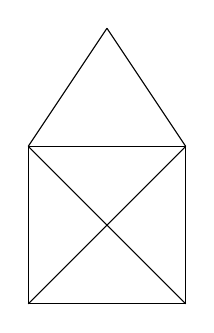
\begin{tikzpicture}
		\draw (0,0) to (0,2);
		\draw (0,2) to (1,3.5);
		\draw (1,3.5) to (2,2);
		\draw (2,2) to (2,0);
		\draw (2,0) to (0,0);
		\draw (0,0) to (2,2);
		\draw (0,2) to (2,0);
		\draw (0,2) to (2,2);
	\end{tikzpicture}
\end{figure}
\end{myTEXEX}
\end{myTEXEXdoclst}

A title can be submitted as an optional argument, which appears in the upper right corner of the box.

\begin{myTEXEXdoclst}{mySTY101}{label={texex:mySTY101}, listing and text}
\begin{myTEXEX}{title={A TIKZ Picture}}
\begin{figure}[H]
	\begin{tikzpicture}
	[...]
	\end{tikzpicture}
\end{figure}
\end{myTEXEX}
\end{myTEXEXdoclst}

By default, the \Verb|myTEXEX| environment does not have syntax highlighting. You can highlight some keywords with the optional \verb|listing options={keywords={}}| argument.

\begin{myTEXEXdoclst}{mySTY102}{label={texex:mySTY102}, listing and text}
\begin{myTEXEX}{title={A TIKZ Picture}, listing options={keywords={tikzpicture}}}
\begin{figure}[H]
	\begin{tikzpicture}
	[...]
	\end{tikzpicture}
\end{figure}
\end{myTEXEX}
\end{myTEXEXdoclst}

If you want to enable line numbering, you can simpy do so with the optional argument \verb|listing options={style=num}|.

\begin{myTEXEXdoclst}{mySTY103}{label={texex:mySTY103}, listing and text}
\begin{myTEXEX}{listing options={style=num, keywords={tikzpicture}}}
\begin{figure}[H]
	\begin{tikzpicture}
	[...]
	\end{tikzpicture}
\end{figure}
\end{myTEXEX}
\end{myTEXEXdoclst}

If you want to show the result of the \LaTeX{} code in the same box, you can do this in different ways.

\begin{myTEXEXdoclst}{mySTY104}{label={texex:mySTY104}, listing and text, listing options={keywords={listing, and, text}}}
\begin{myTEXEX}{listing and text}
\lipsum[4]
\end{myTEXEX}
\end{myTEXEXdoclst}

\begin{myTEXEXdoclst}{mySTY105}{label={texex:mySTY105}, listing and text, listing options={keywords={listing, side, text, center, lower}}}
\begin{myTEXEX}{listing side text, center lower}
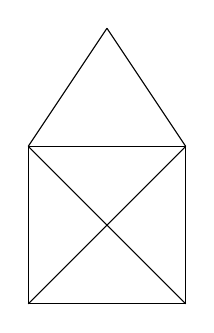
\begin{tikzpicture}
	\draw (0,0) to (0,2);
	\draw (0,2) to (1,3.5);
	\draw (1,3.5) to (2,2);
	\draw (2,2) to (2,0);
	\draw (2,0) to (0,0);
	\draw (0,0) to (2,2);
	\draw (0,2) to (2,0);
	\draw (0,2) to (2,2);
\end{tikzpicture}
\end{myTEXEX}
\end{myTEXEXdoclst}

\begin{myTEXEXdoclst}{mySTY106}{label={texex:mySTY106}, listing and text, listing options={keywords={listing, outside, text, center, lower}}}
\begin{myTEXEX}{listing outside text, center lower}
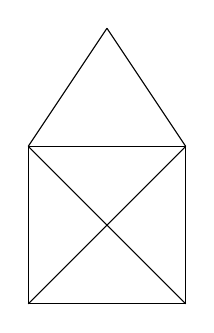
\begin{tikzpicture}
	\draw (0,0) to (0,2);
	\draw (0,2) to (1,3.5);
	\draw (1,3.5) to (2,2);
	\draw (2,2) to (2,0);
	\draw (2,0) to (0,0);
	\draw (0,0) to (2,2);
	\draw (0,2) to (2,0);
	\draw (0,2) to (2,2);
\end{tikzpicture}
\end{myTEXEX}
\end{myTEXEXdoclst}

%
% ####################################################################################################################################################################################
% ####################################################################################################################################################################################
%

\section{The \LaTeX{} Example Environment with a List Index}

The \emph{myTCB-V1} package has a predefined environment, which is called \Verb|myTEXEXlst|. In this environment there is a list index available and listing boxes are created by defalt. A title (\verb|TITLE1|) must be passed as a mandatory argument. This title does not appear on the box, instead it is found in the list index. The box itself is titled with \emph{\LaTeX{} Example} and a sequential number. The main idea for this environment was to build a box that shows the \LaTeX{} code that is located in the body of the document.

\begin{myTEXEXdoclst}{mySTY107}{label={texex:mySTY107}, listing and text}
\begin{myTEXEXlst}{TITLE1}{}
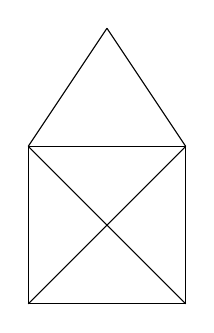
\begin{tikzpicture}
	\draw (0,0) to (0,2);
	\draw (0,2) to (1,3.5);
	\draw (1,3.5) to (2,2);
	\draw (2,2) to (2,0);
	\draw (2,0) to (0,0);
	\draw (0,0) to (2,2);
	\draw (0,2) to (2,0);
	\draw (0,2) to (2,2);
\end{tikzpicture}
\end{myTEXEXlst}
\end{myTEXEXdoclst}

\begin{minipage}{0.46\linewidth}
\centering
\begin{myFIGlst}{myBOX LoF}{label={fig:mytexexlofdef}}
	\includegraphics[page=1,scale=0.18]{examples/myTEXEXV000.pdf}
\end{myFIGlst}
\end{minipage}
\begin{minipage}{0.46\linewidth}
You can create the list index with the command \Verb|\listofmyTEXEX|.

\begin{myTEXEXdoclst}{List Entries of MySTY}{label={texex:mytexexlistentry}, listing only}
\listofmyTEXEX
\end{myTEXEXdoclst}

This will create a list index which looks like the picture in \figref{mytexexlofdef}. 
\end{minipage}

If you want to change the horizontal spacing of the list entries, you can do this quite simple with the following code in the preamble, which is illustrated in \texexref{remleadnumbmytxex}.

\begin{myTEXEXdoclst}{Altering the List Index Spacing of myTEXEXlst}{label={texex:remleadnumbmytxex}, listing only}
\makeatletter
	\renewcommand{\l@myTEXEX}{\@dottedtocline{1}{0mm}{0mm}}
\makeatother
\end{myTEXEXdoclst}

If you want to change the vertical spacing of the list entries, you can do this quite simple with the following code in the preamble, which is illustrated in \texexref{remleadnumbmytxexhori}.

\begin{myTEXEXdoclst}{Altering the List Index Spacing of mySTYlst}{label={texex:remleadnumbmytxexhori}, listing only}
\makeatletter
	\addtocontents{myTEXEX}{\protect\vspace{12mm}}
\makeatother
\end{myTEXEXdoclst}

If you want to get rid of the page numbers in the list index, you can do this quite simple with the following code in the preamble, which is illustrated in \texexref{mytexexnoheadnofoot}.

\begin{myTEXEXdoclst}{myTEXEX no headers}{label={texex:mytexexnoheadnofoot}, listing only}
% copy cmd \listofmyTEXEX into cmd \oldlistofmyTEXEX
\let\oldlistofmyTEXEX\listofmyTEXEX

% renew cmd \listofmyTEXEX
\renewcommand\listofmyTEXEX
{
	\pagestyle{empty} % .... % disable headers/footers
	\oldlistofmyTEXEX % .... % call \oldlistofmyTEXEX
	\clearpage % ........... % create a new page
	\pagestyle{plain} % .... % enable headers/footers; use fancy if you use fancyhdr
}
\end{myTEXEXdoclst}

A label can be specified as an optional argument. The box can then be referenced in the text with \Verb|\texexref{}|.

\begin{myTEXEXdoclst}{myBOX label}{label={texex:mytttttttwithlabel}, listing and text}
\begin{myTEXEXlst}{TITLE2}{label={texex:TEXEXLABEL5}}
\lipsum[4]
\end{myTEXEXlst}
\end{myTEXEXdoclst}

\begin{myTEXEXdoclst}{myBOX label ref}{label={texex:myboxwithlabelref}, listing and text}
This example is shown in \texexref{TEXEXLABEL5}
\end{myTEXEXdoclst}

It is notable that the label has to contain the \Verb|texex:| prefix in order to reference the label appropriately.

By default, the \Verb|myTEXEXlst| environment does not have syntax highlighting. You can highlight some keywords with the optional \verb|listing options={keywords={}}| argument.

\begin{myTEXEXdoclst}{mySTY001}{label={texex:mySTY001}, listing and text}
\begin{myTEXEXlst}{TITLE2}{listing options={keywords={tikzpicture}}}
\begin{figure}[H]
	\begin{tikzpicture}
	[...]
	\end{tikzpicture}
\end{figure}
\end{myTEXEXlst}
\end{myTEXEXdoclst}

If you want to enable line numbering, you can simpy do so with the optional argument \verb|listing options={style=num}|.

\begin{myTEXEXdoclst}{mySTY001}{label={texex:mySTY001}, listing and text}
\begin{myTEXEXlst}{TITLE2}{listing options={style=num, keywords={tikzpicture}}}
\begin{figure}[H]
	\begin{tikzpicture}
	[...]
	\end{tikzpicture}
\end{figure}
\end{myTEXEXlst}
\end{myTEXEXdoclst}

If you want to show the result of the \LaTeX{} code in the same box, you can do this in different ways.

\begin{myTEXEXdoclst}{mySTY001}{label={texex:mySTY001}, listing and text, listing options={keywords={listing, and, text}}}
\begin{myTEXEXlst}{TITLE2}{listing and text}
\lipsum[4]
\end{myTEXEXlst}
\end{myTEXEXdoclst}

\begin{myTEXEXdoclst}{mySTY001}{label={texex:mySTY001}, listing and text, listing options={keywords={listing, side, text, center, lower}}}
\begin{myTEXEXlst}{TITLE2}{listing side text, center lower}
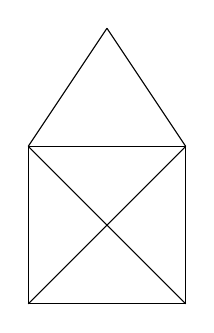
\begin{tikzpicture}
	\draw (0,0) to (0,2);
	\draw (0,2) to (1,3.5);
	\draw (1,3.5) to (2,2);
	\draw (2,2) to (2,0);
	\draw (2,0) to (0,0);
	\draw (0,0) to (2,2);
	\draw (0,2) to (2,0);
	\draw (0,2) to (2,2);
\end{tikzpicture}
\end{myTEXEXlst}
\end{myTEXEXdoclst}

\begin{myTEXEXdoclst}{mySTY001}{label={texex:mySTY001}, listing and text, listing options={keywords={listing, outside, text, center, lower}}}
\begin{myTEXEXlst}{TITLE2}{listing outside text, center lower}
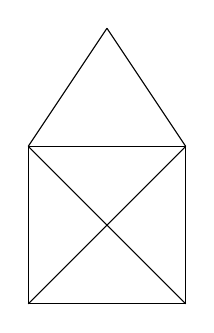
\begin{tikzpicture}
	\draw (0,0) to (0,2);
	\draw (0,2) to (1,3.5);
	\draw (1,3.5) to (2,2);
	\draw (2,2) to (2,0);
	\draw (2,0) to (0,0);
	\draw (0,0) to (2,2);
	\draw (0,2) to (2,0);
	\draw (0,2) to (2,2);
\end{tikzpicture}
\end{myTEXEXlst}
\end{myTEXEXdoclst}

%
% ####################################################################################################################################################################################
% ####################################################################################################################################################################################
%

\section{The Coding Environment without a List Index}

The \emph{myTCB-V1} package has a predefined environment, which is called \Verb|myCODEEX|. In this environment there is no list index available and only listing boxes are created. The main idea for this environment was to build a box that illustriates program code. The programming language should always be passed as an argument (\verb|listing options={language=python}|), even if it is an optional argument.

\begin{myTEXEXdoclst}{mySTY100}{label={texex:mySTY100}, listing and text}
\begin{myCODEEX}{listing options={language=python}}
if a == 5:
	print("HALLO")
\end{myCODEEX}
\end{myTEXEXdoclst}

A title can be submitted as an optional argument, which appears in the upper right corner of the box.

\begin{myTEXEXdoclst}{mySTY100}{label={texex:mySTY100}, listing and text}
\begin{myCODEEX}{title={A simple Python Program}, listing options={language=python}}
if a == 5:
	print("HALLO")
\end{myCODEEX}
\end{myTEXEXdoclst}

If you want to enable line numbering, you can simpy do so with the optional argument \verb|listing options={style=num}|.

\begin{myTEXEXdoclst}{mySTY100}{label={texex:mySTY100}, listing and text}
\begin{myCODEEX}{listing options={language=python, style=num}}
if a == 5:
	print("HALLO")
\end{myCODEEX}
\end{myTEXEXdoclst}

If you want to start with a different line number, you can simpy do so with the optional argument \verb|listing options={firstnumber=88}|.

\begin{myTEXEXdoclst}{mySTY100}{label={texex:mySTY100}, listing and text}
\begin{myCODEEX}{listing options={language=python, style=num, firstnumber=88}}
if a == 5:
	print("HALLO")
\end{myCODEEX}
\end{myTEXEXdoclst}

%
% ####################################################################################################################################################################################
% ####################################################################################################################################################################################
%

\section{The Coding Environment with a List Index}

The \emph{myTCB-V1} package has a predefined environment, which is called \Verb|myCODEEXlst|. In this environment there is a list index available and only listing boxes are created. A title (\verb|TITLE1|) must be passed as a mandatory argument. This title does not appear on the box, instead it is found in the list index. The box itself is titled with \emph{Code Example} and a sequential number. The main idea for this environment was to build a box that illustriates program code. The programming language should always be passed as an argument (\verb|listing options={language=python}|), even if it is an optional argument.

\begin{myTEXEXdoclst}{mySTY100}{label={texex:mySTY100}, listing and text}
\begin{myCODEEXlst}{TITLE1}{listing options={language=python}}
if a == 5:
	print("HALLO")
\end{myCODEEXlst}
\end{myTEXEXdoclst}

\begin{minipage}{0.46\linewidth}
\centering
\begin{myFIGlst}{myBOX LoF}{label={fig:mycodeexlofdef}}
	\includegraphics[page=1,scale=0.18]{examples/myCODEEXV000.pdf}
\end{myFIGlst}
\end{minipage}
\begin{minipage}{0.46\linewidth}
You can create the list index with the command \Verb|\listofmyCODEEX|.

\begin{myTEXEXdoclst}{List Entries of MySTY}{label={texex:mytexexlistentry}, listing only}
\listofmyCODEEX
\end{myTEXEXdoclst}

This will create a list index which looks like the picture in \figref{mycodeexlofdef}. 
\end{minipage}

If you want to change the horizontal spacing of the list entries, you can do this quite simple with the following code in the preamble, which is illustrated in \texexref{remleadnumbmycodeex}.

\begin{myTEXEXdoclst}{Altering the List Index Spacing of myTEXEXlst}{label={texex:remleadnumbmycodeex}, listing only}
\makeatletter
	\renewcommand{\l@myCODEEX}{\@dottedtocline{1}{0mm}{0mm}}
\makeatother
\end{myTEXEXdoclst}

If you want to change the vertical spacing of the list entries, you can do this quite simple with the following code in the preamble, which is illustrated in \texexref{remleadnumbmycodeexhori}.

\begin{myTEXEXdoclst}{Altering the List Index Spacing of mySTYlst}{label={texex:remleadnumbmycodeexhori}, listing only}
\makeatletter
	\addtocontents{myCODEEX}{\protect\vspace{12mm}}
\makeatother
\end{myTEXEXdoclst}

If you want to get rid of the page numbers in the list index, you can do this quite simple with the following code in the preamble, which is illustrated in \texexref{mycodeexnoheadnofoot}.

\begin{myTEXEXdoclst}{myTEXEX no headers}{label={texex:mycodeexnoheadnofoot}, listing only}
% copy cmd \listofmyCODEEX into cmd \oldlistofmyCODEEX
\let\oldlistofmyCODEEX\listofmyCODEEX

% renew cmd \listofmyCODEEX
\renewcommand\listofmyCODEEX
{
	\pagestyle{empty} % .... % disable headers/footers
	\oldlistofmyCODEEX % ... % call \oldlistofmyCODEEX
	\clearpage % ........... % create a new page
	\pagestyle{plain} % .... % enable headers/footers; use fancy if you use fancyhdr
}
\end{myTEXEXdoclst}

A label can be specified as an optional argument. The box can then be referenced in the text with \Verb|\codeexref{}|.

\begin{myTEXEXdoclst}{myBOX label}{label={texex:mytttttttwithlabel}, listing and text}
\begin{myCODEEXlst}{TITLE1}{label={codeex:CODEEXLABEL5}, listing options={language=python}}
if a == 5:
	print("HALLO")
\end{myCODEEXlst}
\end{myTEXEXdoclst}

\begin{myTEXEXdoclst}{myBOX label ref}{label={texex:myboxwithlabelref}, listing and text}
This example is shown in \codeexref{CODEEXLABEL5}
\end{myTEXEXdoclst}

It is notable that the label has to contain the \Verb|codeex:| prefix in order to reference the label appropriately.

If you want to enable line numbering, you can simpy do so with the optional argument \verb|listing options={style=num}|.

\begin{myTEXEXdoclst}{mySTY100}{label={texex:mySTY100}, listing and text}
\begin{myCODEEXlst}{TITLE1}{listing options={language=python, style=num}}
if a == 5:
	print("HALLO")
\end{myCODEEXlst}
\end{myTEXEXdoclst}

If you want to start with a different line number, you can simpy do so with the optional argument \verb|listing options={firstnumber=88}|.

\begin{myTEXEXdoclst}{mySTY100}{label={texex:mySTY100}, listing and text}
\begin{myCODEEXlst}{TITLE1}{listing options={language=python, style=num, firstnumber=88}}
if a == 5:
	print("HALLO")
\end{myCODEEXlst}
\end{myTEXEXdoclst}

%
% ####################################################################################################################################################################################
% ####################################################################################################################################################################################
%

\section{The Configuration Environment without a List Index}

The \emph{myTCB-V1} package has a predefined environment, which is called \Verb|myCONFIGEX|. In this environment there is no list index available and only listing boxes are created. The main idea for this environment was to build a box that shows configuration.

\begin{myTEXEXdoclst}{WHATEVER}{listing and text}
\begin{myCONFIGEX}{}
track at-vie03c-rrINET type route reachability route ipv4 217.25.120.21/32
track at-vie09c-rrINET type route reachability route ipv4 217.25.120.11/32
\end{myCONFIGEX}
\end{myTEXEXdoclst}

A title can be submitted as an optional argument, which appears in the upper right corner of the box.

\begin{myTEXEXdoclst}{mySTY100}{listing and text}
\begin{myCONFIGEX}{title={A simple Tracking Object}}
track at-vie03c-rrINET type route reachability route ipv4 217.25.120.21/32
track at-vie09c-rrINET type route reachability route ipv4 217.25.120.11/32
\end{myCONFIGEX}
\end{myTEXEXdoclst}

If you want to enable line numbering, you can simpy do so with the optional argument \verb|listing options={style=num}|.

\begin{myTEXEXdoclst}{mySTY100}{listing and text}
\begin{myCONFIGEX}{listing options={style=num}}
track at-vie03c-rrINET type route reachability route ipv4 217.25.120.21/32
track at-vie09c-rrINET type route reachability route ipv4 217.25.120.11/32
\end{myCONFIGEX}
\end{myTEXEXdoclst}

If you want to start with a different line number, you can simpy do so with the optional argument \verb|listing options={firstnumber=88}|.

\begin{myTEXEXdoclst}{mySTY100}{listing and text}
\begin{myCONFIGEX}{listing options={style=num, firstnumber=88}}
track at-vie03c-rrINET type route reachability route ipv4 217.25.120.21/32
track at-vie09c-rrINET type route reachability route ipv4 217.25.120.11/32
\end{myCONFIGEX}
\end{myTEXEXdoclst}

By default, the \Verb|myCONFIGEX| environment does not have syntax highlighting. You can highlight some keywords with the optional \verb|listing options={keywords={}}| argument.

\begin{myTEXEXdoclst}{mySTY220}{listing and text}
\begin{myCONFIGEX}{listing options={style=num, keywords={track}}}
track at-vie03c-rrINET type route reachability route ipv4 217.25.120.21/32
track at-vie09c-rrINET type route reachability route ipv4 217.25.120.11/32
\end{myCONFIGEX}
\end{myTEXEXdoclst}

You can even use \LaTeX Code within the \Verb|myCONFIGEX| environment with the default escapecharacter \Verb|&|.

\begin{myTEXEXdoclst}{mySTY220}{listing and text, listing options={escapechar=\#}}
\begin{myCONFIGEX}{listing options={style=num}}
track at-vie03c-rrINET type &{\color{red}route}& reachability route ipv4 217.25.120.21/32
track at-vie09c-rrINET type route reachability route ipv4 217.25.120.11/32
\end{myCONFIGEX}
\end{myTEXEXdoclst}

\DefineShortVerb{\#}

This can be changed with the optional \verb#listing options={escapechar=\|}# argument.

\begin{myTEXEXdoclst}{mySTY220}{listing and text, listing options={escapechar=\#}}
\begin{myCONFIGEX}{listing options={style=num, escapechar=\|}}
track at-vie03c-rrINET type |{\color{red}route}| reachability route ipv4 217.25.120.21/32
track at-vie09c-rrINET type route reachability route ipv4 217.25.120.11/32
\end{myCONFIGEX}
\end{myTEXEXdoclst}

%
% ####################################################################################################################################################################################
% ####################################################################################################################################################################################
%

\section{The Configuration Environment with a List Index}

The \emph{myTCB-V1} package has a predefined environment, which is called \Verb|myCONFIGEXlst|. In this environment there is a list index available and only listing boxes are created. A title (\verb|TITLE1|) must be passed as a mandatory argument. This title does not appear on the box, instead it is found in the list index. The box itself is titled with \emph{Configuration Example} and a sequential number. The main idea for this environment was to build a box that shows configuration.

\begin{myTEXEXdoclst}{mySTY100}{listing and text}
\begin{myCONFIGEXlst}{TITLE1}{}
track at-vie03c-rrINET type route reachability route ipv4 217.25.120.21/32
track at-vie09c-rrINET type route reachability route ipv4 217.25.120.11/32
\end{myCONFIGEXlst}
\end{myTEXEXdoclst}

\begin{minipage}{0.46\linewidth}
\centering
\begin{myFIGlst}{myBOX LoF}{label={fig:myCONFIGEXlofdef}}
	\includegraphics[page=1,scale=0.18]{examples/myCONFIGEXV000.pdf}
\end{myFIGlst}
\end{minipage}
\begin{minipage}{0.46\linewidth}
You can create the list index with the command \Verb|\listofmyCONFIGEX|.

\begin{myTEXEXdoclst}{List Entries of MySTY}{listing only}
\listofmyCONFIGEX
\end{myTEXEXdoclst}

This will create a list index which looks like the picture in \figref{myCONFIGEXlofdef}. 
\end{minipage}

If you want to change the horizontal spacing of the list entries, you can do this quite simple with the following code in the preamble, which is illustrated in \texexref{remleadnumbmyCONFIGEX}.

\begin{myTEXEXdoclst}{Altering the List Index Spacing of myTEXEXlst}{label={texex:remleadnumbmyCONFIGEX}, listing only}
\makeatletter
	\renewcommand{\l@myCONFIGEX}{\@dottedtocline{1}{0mm}{0mm}}
\makeatother
\end{myTEXEXdoclst}

If you want to change the vertical spacing of the list entries, you can do this quite simple with the following code in the preamble, which is illustrated in \texexref{remleadnumbmyCONFIGEXhori}.

\begin{myTEXEXdoclst}{Altering the List Index Spacing of mySTYlst}{label={texex:remleadnumbmyCONFIGEXhori}, listing only}
\makeatletter
	\addtocontents{myCONFIGEX}{\protect\vspace{12mm}}
\makeatother
\end{myTEXEXdoclst}

If you want to get rid of the page numbers in the list index, you can do this quite simple with the following code in the preamble, which is illustrated in \texexref{myCONFIGEXnoheadnofoot}.

\begin{myTEXEXdoclst}{myTEXEX no headers}{label={texex:myCONFIGEXnoheadnofoot}, listing only}
% copy cmd \listofmyCONFIGEX into cmd \oldlistofmyCONFIGEX
\let\oldlistofmyCONFIGEX\listofmyCONFIGEX

% renew cmd \listofmyCONFIGEX
\renewcommand\listofmyCONFIGEX
{
	\pagestyle{empty} % ...... % disable headers/footers
	\oldlistofmyCONFIGEX % ... % call \oldlistofmyCONFIGEX
	\clearpage % ............. % create a new page
	\pagestyle{plain} % ...... % enable headers/footers; use fancy if you use fancyhdr
}
\end{myTEXEXdoclst}

A label can be specified as an optional argument. The box can then be referenced in the text with \Verb|\configexref{}|.

\begin{myTEXEXdoclst}{myBOX label}{label={texex:mytttttttwithlabel}, listing and text}
\begin{myCONFIGEXlst}{TITLE1}{label={configex:CONFIGEXLABEL5}}
track at-vie03c-rrINET type route reachability route ipv4 217.25.120.21/32
track at-vie09c-rrINET type route reachability route ipv4 217.25.120.11/32
\end{myCONFIGEXlst}
\end{myTEXEXdoclst}

\begin{myTEXEXdoclst}{myBOX label ref}{label={texex:myboxwithlabelref}, listing and text}
This example is shown in \configexref{CONFIGEXLABEL5}
\end{myTEXEXdoclst}

It is notable that the label has to contain the \Verb|configex:| prefix in order to reference the label appropriately.

If you want to enable line numbering, you can simpy do so with the optional argument \verb|listing options={style=num}|.

\begin{myTEXEXdoclst}{mySTY100}{label={texex:mySTY100}, listing and text}
\begin{myCONFIGEXlst}{TITLE1}{listing options={style=num}}
track at-vie03c-rrINET type route reachability route ipv4 217.25.120.21/32
track at-vie09c-rrINET type route reachability route ipv4 217.25.120.11/32
\end{myCONFIGEXlst}
\end{myTEXEXdoclst}

If you want to start with a different line number, you can simpy do so with the optional argument \verb|listing options={firstnumber=88}|.

\begin{myTEXEXdoclst}{mySTY100}{label={texex:mySTY100}, listing and text}
\begin{myCONFIGEXlst}{TITLE1}{listing options={style=num, firstnumber=88}}
track at-vie03c-rrINET type route reachability route ipv4 217.25.120.21/32
track at-vie09c-rrINET type route reachability route ipv4 217.25.120.11/32
\end{myCONFIGEXlst}
\end{myTEXEXdoclst}

By default, the \Verb|myCONFIGEX| environment does not have syntax highlighting. You can highlight some keywords with the optional \verb|listing options={keywords={}}| argument.

\begin{myTEXEXdoclst}{mySTY220}{listing and text}
\begin{myCONFIGEXlst}{TITLE1}{listing options={style=num, keywords={track}}}
track at-vie03c-rrINET type route reachability route ipv4 217.25.120.21/32
track at-vie09c-rrINET type route reachability route ipv4 217.25.120.11/32
\end{myCONFIGEXlst}
\end{myTEXEXdoclst}

You can even use \LaTeX Code within the \Verb|myCONFIGEX| environment with the default escapecharacter \Verb|&|.

\begin{myTEXEXdoclst}{mySTY220}{listing and text, listing options={escapechar=\#}}
\begin{myCONFIGEXlst}{TITLE1}{listing options={style=num}}
track at-vie03c-rrINET type &{\color{red}route}& reachability route ipv4 217.25.120.21/32
track at-vie09c-rrINET type route reachability route ipv4 217.25.120.11/32
\end{myCONFIGEXlst}
\end{myTEXEXdoclst}

This can be changed with the optional \verb#listing options={escapechar=\|}# argument.

\begin{myTEXEXdoclst}{mySTY220}{listing and text, listing options={escapechar=\#}}
\begin{myCONFIGEXlst}{TITLE1}{listing options={style=num, escapechar=\|}}
track at-vie03c-rrINET type |{\color{red}route}| reachability route ipv4 217.25.120.21/32
track at-vie09c-rrINET type route reachability route ipv4 217.25.120.11/32
\end{myCONFIGEXlst}
\end{myTEXEXdoclst}

%
% ####################################################################################################################################################################################
% ####################################################################################################################################################################################
%

\section{The File Environment without a List Index}

The \emph{myTCB-V1} package has a predefined environment, which is called \Verb|myFILE|. In this environment there is no list index available and only listing boxes are created. The main idea for this environment was to build a box that shows file content.

\begin{myTEXEXdoclst}{WHATEVER}{listing and text}
\begin{myFILE}{}
<VirtualHost 192.168.1.1 172.20.30.40>
	DocumentRoot "/www/server1"
	ServerName server.example.com
</VirtualHost>
\end{myFILE}
\end{myTEXEXdoclst}

A title can be submitted as an optional argument, which appears in the upper right corner of the box.

\begin{myTEXEXdoclst}{mySTY100}{listing and text}
\begin{myFILE}{title={A simple Apache Configuration}}
<VirtualHost 192.168.1.1 172.20.30.40>
	DocumentRoot "/www/server1"
	ServerName server.example.com
</VirtualHost>
\end{myFILE}
\end{myTEXEXdoclst}

If you want to enable line numbering, you can simpy do so with the optional argument \verb|listing options={style=num}|.

\begin{myTEXEXdoclst}{mySTY100}{listing and text}
\begin{myFILE}{listing options={style=num}}
<VirtualHost 192.168.1.1 172.20.30.40>
	DocumentRoot "/www/server1"
	ServerName server.example.com
</VirtualHost>
\end{myFILE}
\end{myTEXEXdoclst}

If you want to start with a different line number, you can simpy do so with the optional argument \verb|listing options={firstnumber=88}|.

\begin{myTEXEXdoclst}{mySTY100}{listing and text}
\begin{myFILE}{listing options={style=num, firstnumber=88}}
<VirtualHost 192.168.1.1 172.20.30.40>
	DocumentRoot "/www/server1"
	ServerName server.example.com
</VirtualHost>
\end{myFILE}
\end{myTEXEXdoclst}

By default, the \Verb|myFILE| environment does not have syntax highlighting. You can highlight some keywords with the optional \verb|listing options={keywords={}}| argument.

\begin{myTEXEXdoclst}{mySTY220}{listing and text}
\begin{myFILE}{listing options={style=num, keywords={ServerName}}}
<VirtualHost 192.168.1.1 172.20.30.40>
	DocumentRoot "/www/server1"
	ServerName server.example.com
</VirtualHost>
\end{myFILE}
\end{myTEXEXdoclst}

You can even use \LaTeX Code within the \Verb|myFILE| environment with the default escapecharacter \Verb|&|.

\begin{myTEXEXdoclst}{mySTY220}{listing and text, listing options={escapechar=\#}}
\begin{myFILE}{listing options={style=num}}
<VirtualHost 192.168.1.1 172.20.30.40>
	DocumentRoot "/www/server1"
	ServerName &{\color{red}server.example.com}&
</VirtualHost>
\end{myFILE}
\end{myTEXEXdoclst}

This can be changed with the optional \verb#listing options={escapechar=\|}# argument.

\begin{myTEXEXdoclst}{mySTY220}{listing and text, listing options={escapechar=\#}}
\begin{myFILE}{listing options={style=num, escapechar=\|}}
<VirtualHost 192.168.1.1 172.20.30.40>
	DocumentRoot "/www/server1"
	ServerName |{\color{red}server.example.com}|
</VirtualHost>
\end{myFILE}
\end{myTEXEXdoclst}

%
% ####################################################################################################################################################################################
% ####################################################################################################################################################################################
%

\section{The File Environment with a List Index}

The \emph{myTCB-V1} package has a predefined environment, which is called \Verb|myFILElst|. In this environment there is a list index available and only listing boxes are created. A title (\verb|TITLE1|) must be passed as a mandatory argument. This title does not appear on the box, instead it is found in the list index. The box itself is titled with \emph{File Example} and a sequential number. The main idea for this environment was to build a box that shows file content.

\begin{myTEXEXdoclst}{mySTY100}{listing and text}
\begin{myFILElst}{TITLE1}{}
<VirtualHost 192.168.1.1 172.20.30.40>
	DocumentRoot "/www/server1"
	ServerName server.example.com
</VirtualHost>
\end{myFILElst}
\end{myTEXEXdoclst}

\begin{minipage}{0.46\linewidth}
\centering
\begin{myFIGlst}{myBOX LoF}{label={fig:myFILElofdef}}
	\includegraphics[page=1,scale=0.18]{examples/myFILEV000.pdf}
\end{myFIGlst}
\end{minipage}
\begin{minipage}{0.46\linewidth}
You can create the list index with the command \Verb|\listofmyFILE|.

\begin{myTEXEXdoclst}{List Entries of MySTY}{listing only}
\listofmyFILE
\end{myTEXEXdoclst}

This will create a list index which looks like the picture in \figref{myFILElofdef}. 
\end{minipage}

If you want to change the horizontal spacing of the list entries, you can do this quite simple with the following code in the preamble, which is illustrated in \texexref{remleadnumbmyFILE}.

\begin{myTEXEXdoclst}{Altering the List Index Spacing of myTEXEXlst}{label={texex:remleadnumbmyFILE}, listing only}
\makeatletter
	\renewcommand{\l@myFILE}{\@dottedtocline{1}{0mm}{0mm}}
\makeatother
\end{myTEXEXdoclst}

If you want to change the vertical spacing of the list entries, you can do this quite simple with the following code in the preamble, which is illustrated in \texexref{remleadnumbmyFILEhori}.

\begin{myTEXEXdoclst}{Altering the List Index Spacing of mySTYlst}{label={texex:remleadnumbmyFILEhori}, listing only}
\makeatletter
	\addtocontents{myFILE}{\protect\vspace{12mm}}
\makeatother
\end{myTEXEXdoclst}

If you want to get rid of the page numbers in the list index, you can do this quite simple with the following code in the preamble, which is illustrated in \texexref{myFILEnoheadnofoot}.

\begin{myTEXEXdoclst}{myTEXEX no headers}{label={texex:myFILEnoheadnofoot}, listing only}
% copy cmd \listofmyFILE into cmd \oldlistofmyFILE
\let\oldlistofmyFILE\listofmyFILE

% renew cmd \listofmyFILE
\renewcommand\listofmyFILE
{
	\pagestyle{empty} % ...... % disable headers/footers
	\oldlistofmyFILE % ....... % call \oldlistofmyFILE
	\clearpage % ............. % create a new page
	\pagestyle{plain} % ...... % enable headers/footers; use fancy if you use fancyhdr
}
\end{myTEXEXdoclst}

A label can be specified as an optional argument. The box can then be referenced in the text with \Verb|\fileref{}|.

\begin{myTEXEXdoclst}{myBOX label}{label={texex:mytttttttwithlabel}, listing and text}
\begin{myFILElst}{TITLE1}{label={file:FILELABEL5}}
<VirtualHost 192.168.1.1 172.20.30.40>
	DocumentRoot "/www/server1"
	ServerName server.example.com
	</VirtualHost>
\end{myFILElst}
\end{myTEXEXdoclst}

\begin{myTEXEXdoclst}{myBOX label ref}{label={texex:myboxwithlabelref}, listing and text}
This is shown in \fileref{FILELABEL5}
\end{myTEXEXdoclst}

It is notable that the label has to contain the \Verb|file:| prefix in order to reference the label appropriately.

If you want to enable line numbering, you can simpy do so with the optional argument \verb|listing options={style=num}|.

\begin{myTEXEXdoclst}{mySTY100}{label={texex:mySTY100}, listing and text}
\begin{myFILElst}{TITLE1}{listing options={style=num}}
<VirtualHost 192.168.1.1 172.20.30.40>
	DocumentRoot "/www/server1"
	ServerName server.example.com
</VirtualHost>
\end{myFILElst}
\end{myTEXEXdoclst}

If you want to start with a different line number, you can simpy do so with the optional argument \verb|listing options={firstnumber=88}|.

\begin{myTEXEXdoclst}{mySTY100}{label={texex:mySTY100}, listing and text}
\begin{myFILElst}{TITLE1}{listing options={style=num, firstnumber=88}}
<VirtualHost 192.168.1.1 172.20.30.40>
	DocumentRoot "/www/server1"
	ServerName server.example.com
</VirtualHost>
\end{myFILElst}
\end{myTEXEXdoclst}

By default, the \Verb|myFILE| environment does not have syntax highlighting. You can highlight some keywords with the optional \verb|listing options={keywords={}}| argument.

\begin{myTEXEXdoclst}{mySTY220}{listing and text}
\begin{myFILElst}{TITLE1}{listing options={style=num, keywords={ServerName}}}
<VirtualHost 192.168.1.1 172.20.30.40>
	DocumentRoot "/www/server1"
	ServerName server.example.com
</VirtualHost>
\end{myFILElst}
\end{myTEXEXdoclst}

You can even use \LaTeX Code within the \Verb|myFILE| environment with the default escapecharacter \Verb|&|.

\begin{myTEXEXdoclst}{mySTY220}{listing and text, listing options={escapechar=\#}}
\begin{myFILElst}{TITLE1}{listing options={style=num}}
<VirtualHost 192.168.1.1 172.20.30.40>
	DocumentRoot "/www/server1"
	ServerName &{\color{red}server.example.com}&
</VirtualHost>
\end{myFILElst}
\end{myTEXEXdoclst}

This can be changed with the optional \verb#listing options={escapechar=\|}# argument.

\begin{myTEXEXdoclst}{mySTY220}{listing and text, listing options={escapechar=\#}}
\begin{myFILElst}{TITLE1}{listing options={style=num, escapechar=\|}}
<VirtualHost 192.168.1.1 172.20.30.40>
	DocumentRoot "/www/server1"
	ServerName |{\color{red}server.example.com}|
</VirtualHost>
\end{myFILElst}
\end{myTEXEXdoclst}

%
% ####################################################################################################################################################################################
% ####################################################################################################################################################################################
%

\section{The Output Environment without a List Index}

The \emph{myTCB-V1} package has a predefined environment, which is called \Verb|myOUT|. In this environment there is no list index available and only listing boxes are created. The main idea for this environment was to build a box that shows the output of a command.

\begin{myTEXEXdoclst}{WHATEVER}{listing and text}
\begin{myOUT}{}
This file was created automatically from
a shell script
\end{myOUT}
\end{myTEXEXdoclst}

A title can be submitted as an optional argument, which appears in the upper right corner of the box.

\begin{myTEXEXdoclst}{mySTY100}{listing and text}
\begin{myOUT}{title={A simple Command Output}}
This file was created automatically from
a shell script
\end{myOUT}
\end{myTEXEXdoclst}

If you want to enable line numbering, you can simpy do so with the optional argument \verb|listing options={style=num}|.

\begin{myTEXEXdoclst}{mySTY100}{listing and text}
\begin{myOUT}{listing options={style=num}}
This file was created automatically from
a shell script
\end{myOUT}
\end{myTEXEXdoclst}

If you want to start with a different line number, you can simpy do so with the optional argument \verb|listing options={firstnumber=88}|.

\begin{myTEXEXdoclst}{mySTY100}{listing and text}
\begin{myOUT}{listing options={style=num, firstnumber=88}}
This file was created automatically from
a shell script
\end{myOUT}
\end{myTEXEXdoclst}

By default, the \Verb|myOUT| environment does not have syntax highlighting. You can highlight some keywords with the optional \verb|listing options={keywords={}}| argument.

\begin{myTEXEXdoclst}{mySTY220}{listing and text}
\begin{myOUT}{listing options={style=num, keywords={ServerName}}}
This file was created automatically from
a shell script
\end{myOUT}
\end{myTEXEXdoclst}

You can even use \LaTeX Code within the \Verb|myOUT| environment with the default escapecharacter \Verb|&|.

\begin{myTEXEXdoclst}{mySTY220}{listing and text, listing options={escapechar=\#}}
\begin{myOUT}{listing options={style=num}}
This file was created &{\color{red}automatically}& from
a shell script
\end{myOUT}
\end{myTEXEXdoclst}

This can be changed with the optional \verb#listing options={escapechar=\|}# argument.

\begin{myTEXEXdoclst}{mySTY220}{listing and text, listing options={escapechar=\#}}
\begin{myOUT}{listing options={style=num, escapechar=\|}}
This file was created |{\color{red}automatically}| from
a shell script
\end{myOUT}
\end{myTEXEXdoclst}

%
% ####################################################################################################################################################################################
% ####################################################################################################################################################################################
%

\section{The Output Environment with a List Index}

The \emph{myTCB-V1} package has a predefined environment, which is called \Verb|myOUTlst|. In this environment there is a list index available and only listing boxes are created. A title (\verb|TITLE1|) must be passed as a mandatory argument. This title does not appear on the box, instead it is found in the list index. The box itself is titled with \emph{OUTPUT Example} and a sequential number. The main idea for this environment was to build a box that shows the output of a command.

\begin{myTEXEXdoclst}{mySTY100}{listing and text}
\begin{myOUTlst}{TITLE1}{}
This file was created automatically from
a shell script
\end{myOUTlst}
\end{myTEXEXdoclst}

\begin{minipage}{0.46\linewidth}
\centering
\begin{myFIGlst}{myBOX LoF}{label={fig:myOUTlofdef}}
	\includegraphics[page=1,scale=0.18]{examples/myOUTV000.pdf}
\end{myFIGlst}
\end{minipage}
\begin{minipage}{0.46\linewidth}
You can create the list index with the command \Verb|\listofmyOUT|.

\begin{myTEXEXdoclst}{List Entries of MySTY}{listing only}
\listofmyOUT
\end{myTEXEXdoclst}

This will create a list index which looks like the picture in \figref{myOUTlofdef}. 
\end{minipage}

If you want to change the horizontal spacing of the list entries, you can do this quite simple with the following code in the preamble, which is illustrated in \texexref{remleadnumbmyOUT}.

\begin{myTEXEXdoclst}{Altering the List Index Spacing of myTEXEXlst}{label={texex:remleadnumbmyOUT}, listing only}
\makeatletter
	\renewcommand{\l@myOUT}{\@dottedtocline{1}{0mm}{0mm}}
\makeatother
\end{myTEXEXdoclst}

If you want to change the vertical spacing of the list entries, you can do this quite simple with the following code in the preamble, which is illustrated in \texexref{remleadnumbmyOUThori}.

\begin{myTEXEXdoclst}{Altering the List Index Spacing of mySTYlst}{label={texex:remleadnumbmyOUThori}, listing only}
\makeatletter
	\addtocontents{myOUT}{\protect\vspace{12mm}}
\makeatother
\end{myTEXEXdoclst}

If you want to get rid of the page numbers in the list index, you can do this quite simple with the following code in the preamble, which is illustrated in \texexref{myOUTnoheadnofoot}.

\begin{myTEXEXdoclst}{myTEXEX no headers}{label={texex:myOUTnoheadnofoot}, listing only}
% copy cmd \listofmyOUT into cmd \oldlistofmyOUT
\let\oldlistofmyOUT\listofmyOUT
	
% renew cmd \listofmyOUT
\renewcommand\listofmyOUT
{
	\pagestyle{empty} % ...... % disable headers/footers
	\oldlistofmyOUT % ........ % call \oldlistofmyOUT
	\clearpage % ............. % create a new page
	\pagestyle{plain} % ...... % enable headers/footers; use fancy if you use fancyhdr
}
\end{myTEXEXdoclst}

A label can be specified as an optional argument. The box can then be referenced in the text with \Verb|\outref{}|.

\begin{myTEXEXdoclst}{myBOX label}{label={texex:mytttttttwithlabel}, listing and text}
\begin{myOUTlst}{TITLE1}{label={out:OUTLABEL5}}
This file was created automatically from
a shell script
\end{myOUTlst}
\end{myTEXEXdoclst}

\begin{myTEXEXdoclst}{myBOX label ref}{label={texex:myboxwithlabelref}, listing and text}
This is shown in \outref{OUTLABEL5}
\end{myTEXEXdoclst}

It is notable that the label has to contain the \Verb|out:| prefix in order to reference the label appropriately.

If you want to enable line numbering, you can simpy do so with the optional argument \verb|listing options={style=num}|.

\begin{myTEXEXdoclst}{mySTY100}{label={texex:mySTY100}, listing and text}
\begin{myOUTlst}{TITLE1}{listing options={style=num}}
This file was created automatically from
a shell script
\end{myOUTlst}
\end{myTEXEXdoclst}

If you want to start with a different line number, you can simpy do so with the optional argument \verb|listing options={firstnumber=88}|.

\begin{myTEXEXdoclst}{mySTY100}{label={texex:mySTY100}, listing and text}
\begin{myOUTlst}{TITLE1}{listing options={style=num, firstnumber=88}}
This file was created automatically from
a shell script
\end{myOUTlst}
\end{myTEXEXdoclst}

By default, the \Verb|myOUT| environment does not have syntax highlighting. You can highlight some keywords with the optional \verb|listing options={keywords={}}| argument.

\begin{myTEXEXdoclst}{mySTY220}{listing and text}
\begin{myOUTlst}{TITLE1}{listing options={style=num, keywords={was}}}
This file was created automatically from
a shell script
\end{myOUTlst}
\end{myTEXEXdoclst}

You can even use \LaTeX Code within the \Verb|myOUT| environment with the default escapecharacter \Verb|&|.

\begin{myTEXEXdoclst}{mySTY220}{listing and text, listing options={escapechar=\#}}
\begin{myOUTlst}{TITLE1}{listing options={style=num}}
This file was created &{\color{red}automatically}& from
a shell script
\end{myOUTlst}
\end{myTEXEXdoclst}

This can be changed with the optional \verb#listing options={escapechar=\|}# argument.

\begin{myTEXEXdoclst}{mySTY220}{listing and text, listing options={escapechar=\#}}
\begin{myOUTlst}{TITLE1}{listing options={style=num, escapechar=\|}}
This file was created |{\color{red}automatically}| from
a shell script
\end{myOUTlst}
\end{myTEXEXdoclst}

%
% ####################################################################################################################################################################################
% ####################################################################################################################################################################################
%

\clearpage
\pagestyle{empty}
\printbibliography[heading=bibnumbered]
\clearpage
\pagestyle{plain}

%
% ####################################################################################################################################################################################
% ####################################################################################################################################################################################
%

\end{document}

%
% ####################################################################################################################################################################################
% ####################################################################################################################################################################################
% ####################################################################################################################################################################################
% ####################################################################################################################################################################################
%